\chapter{Methods}

The aim of this thesis is to use inverse design to find a phononic beamsplitter,
a task that can be divided into three parts: 
First, some definitions of what
should be designed and what constitutes a ``good'' design needs to be made.
Second, we need a way to calculate the gradient of the ``goodness'' with respect
to the design.
And lastly, we need a gradient based optimization algorithm to find the optimal
design.
All of this will be described in this chapter.

\section{Design}

The device design to be optimized can be seen in figure~\ref{fig:bs-design}

\begin{figure}[htpb]
	\centering
	\def \a{0.5}
\def \w{1.0}
\def \hx{0.13}
\def \hy{0.3}

\tikzset{
	unitcell/.pic={
		\draw[pic actions] (-0.5*\a, -0.5*\w) rectangle (0.5*\a, 0.5*\w);
		\draw[fill=white] (0, 0) circle [x radius=\hx, y radius=\hy];
	}
}

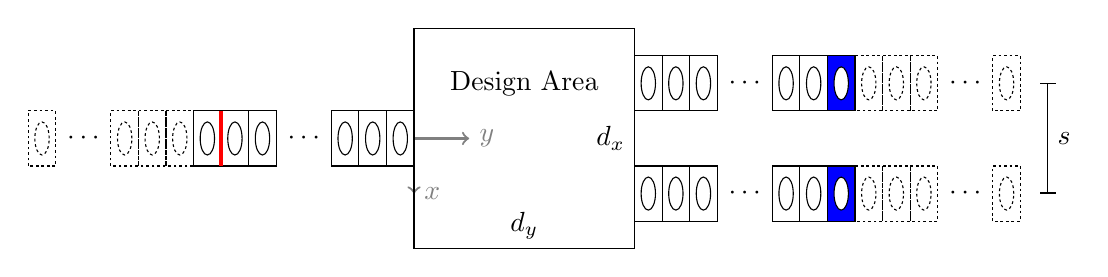
\begin{tikzpicture}[scale=0.7]
	\def \designx{4.0}
	\def \designy{4.0}
	\def \outputh{1.0}
	\def \nunitcells{16}
	\def \nnonpmls{10}

	% Coordinate system
	\draw[gray, thick, ->] (0,0) -- (0,-1) node [anchor=west] {$x$};
	\draw[gray, thick, ->] (0,0) -- (1,0) node [anchor=west] {$y$};

	% Input waveguide
	\path
		(-0.5*\a, 0) pic[transform shape] {unitcell}
		(-1.5*\a, 0) pic[transform shape] {unitcell}
		(-2.5*\a, 0) pic[transform shape] {unitcell}
		(-4.0*\a, 0) node {$\cdots$}
		(-5.5*\a, 0) pic[transform shape] {unitcell}
		(-6.5*\a, 0) pic[transform shape] {unitcell}
		(-7.5*\a, 0) pic[transform shape] {unitcell};
	\draw[red, ultra thick]
		(-7*\a, -0.5*\w) --
		(-7*\a, +0.5*\w);
	\begin{scope}[dash=on 1pt off 1pt phase 0pt]
	\path
		(-8.5*\a, 0) pic[transform shape] {unitcell}
		(-9.5*\a, 0) pic[transform shape] {unitcell}
		(-10.5*\a, 0) pic[transform shape] {unitcell}
		(-12.0*\a, 0) node {$\cdots$}
		(-13.5*\a, 0) pic[transform shape] {unitcell};
	\end{scope}

	% Design area
	\draw (0, -\designx / 2) rectangle (\designy, \designx / 2);
	\node at (\designy / 2, 1) {Design Area};
	\node[left] at (\designy, 0) {$d_x$};
	\node[above] at (\designy/2, -\designx/2) {$d_y$};

	% Output waveguide
	\begin{scope}[xshift=\designy cm, yshift=\outputh cm]
	\path
		(0.5*\a, 0) pic[transform shape] {unitcell}
		(1.5*\a, 0) pic[transform shape] {unitcell}
		(2.5*\a, 0) pic[transform shape] {unitcell}
		(4.0*\a, 0) node {$\cdots$}
		(5.5*\a, 0) pic[transform shape] {unitcell}
		(6.5*\a, 0) pic[transform shape] {unitcell}
		(7.5*\a, 0) pic[transform shape, fill=blue] {unitcell};
	\begin{scope}[dash=on 1pt off 1pt phase 0pt]
	\path
		(8.5*\a, 0) pic[transform shape] {unitcell}
		(9.5*\a, 0) pic[transform shape] {unitcell}
		(10.5*\a, 0) pic[transform shape] {unitcell}
		(12.0*\a, 0) node {$\cdots$}
		(13.5*\a, 0) pic[transform shape] {unitcell};
	\end{scope}
	\end{scope}
	\begin{scope}[xshift=\designy cm, yshift=-\outputh cm]
	\path
		(0.5*\a, 0) pic[transform shape] {unitcell}
		(1.5*\a, 0) pic[transform shape] {unitcell}
		(2.5*\a, 0) pic[transform shape] {unitcell}
		(4.0*\a, 0) node {$\cdots$}
		(5.5*\a, 0) pic[transform shape] {unitcell}
		(6.5*\a, 0) pic[transform shape] {unitcell}
		(7.5*\a, 0) pic[transform shape, fill=blue] {unitcell};
	\begin{scope}[dash=on 1pt off 1pt phase 0pt]
	\path
		(8.5*\a, 0) pic[transform shape] {unitcell}
		(9.5*\a, 0) pic[transform shape] {unitcell}
		(10.5*\a, 0) pic[transform shape] {unitcell}
		(12.0*\a, 0) node {$\cdots$}
		(13.5*\a, 0) pic[transform shape] {unitcell};
	\end{scope}
	\end{scope}
	\draw[|-|]
		(15*\a + \designy, -\outputh) -- node[right] {$s$}
		(15*\a + \designy, \outputh);
		
\end{tikzpicture}

	\caption{
		Device design to be optimized.
		At the red line, a wave traveling right is excited.
		On the blue unit cells is where the output is measured.
		The dashed unit cells are \gls{pml}
	}
	\label{fig:bs-design}
\end{figure}

\tododec{Write about why we use the mode we use, and why I clamp the bottom. Can
reference Johan and Pauls paper}

\subsection{Perfectly Matched Layers (PMLs)}

Ideally, we would like to have infinite waveguides but that cannot be done in
practice.
Instead, \glspl{pml} are placed at the caps of the input and output waveguides.
The purpose of the \gls{pml} is to absorb any incoming waves without reflection,
which would make it act as if there was an infinite waveguide on the other side
into which the waves propagate indefinitely.
The way to accomplish this is to add an imaginary component to the density of
the material.
If there is an abrupt transition from a real density to a significant imaginary
part, reflections will be created at that transition instead.
Therefore, the imaginary part is taken to be exponentially increasing:
\begin{equation}
	\rho_\text{im} = \rho_\text{si} \cdot s \cdot e^{-\abs{y-y_0} / d}
\end{equation}

\begin{figure}[htpb]
	\centering
	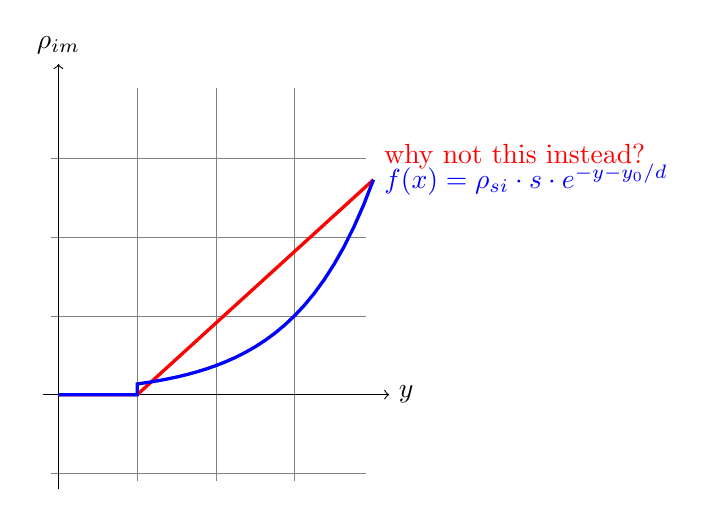
\begin{tikzpicture}[domain=1:4]
		\draw[very thin,color=gray] (-0.1,-1.1) grid (3.9,3.9);

		\draw[->] (-0.2,0) -- (4.2,0) node[right] {$y$};
		\draw[->] (0,-1.2) -- (0,4.2) node[above] {$\rho_\text{im}$};
		\draw[color=red, very thick] (0,0) -- (1,0) -- plot (\x,{(\x-1) *
			0.05*exp(4) / 3})
			node[anchor=south west] {why not this instead?};
		\draw[color=blue, very thick] (0,0) -- (1,0) -- plot (\x,{0.05*exp(\x)})
			node[right] {$f(x) = \rho_\text{si} \cdot s \cdot e^{-\abs{y-y_0} / d}$};
	\end{tikzpicture}
	\caption{Profile of the imaginary component of the waveguides}
	\label{fig:}
\end{figure}

\todoblk{Hold up\ldots why do I choose an exponentially increasing imaginary
	component. If the two possible sources of reflections are the discontinuous
	jump when the pml starts and that the increase is too steep, then why not
	just use a straight line?
}


\subsection{Level-set}

\todowrt{Description of what level-set is: A way of storing a boundary between
two regions; and how it works: Signed distance function}

\todowrt{Description of it's advantages: Easily evolved (level-set equation), no
connectivity issues, see level-set book}

\tododec{Write about how I use it? This feels like it should come after I've
talked about computing the derivative.}

\subsection{Objective function}

\tododec{Maybe I'll only mention that $f$ is an integral of the displacement
	field in the theory and here give the specific formula:
}
\begin{equation}
	\fobj = \int_{\Omega_1} \vec{m_1}^*(\vec{x}) \vec{u}(\vec{x})
	\dl{x} + \int_{\Omega_2} \vec{m_2}^*(\vec{x}) \vec{u}(\vec{x})
\end{equation}

\tododec{Paragraph about pure part of objective function, enforcing the minimum
feature size}

\section{Adjoint Simulation}

\tododec{Give the explicit formula for the gradient now that the objective
function has been fully defined}

\section{Optimization}

\tododec{Describe what optimization algorithm was used, as well as how this
	changed during the simulation. E.g.\ first 200 iterations ADAM; next ADAM
	but with sigmoid function application; sigmoid + feature size; and finally level-set.
}
